\chapter{Datové formáty pro ukládání rentgenových snímků}
Datové formáty pro ukládání rentgenových se vyvíjely společně s vývojem radiografických technologií. S příchodem digitálních technologií pro snímání rentgenových snímků bylo nutné navrhnout standard, který umožní ukládat, přenášet a zálohovat rentgenové snímky společně s jejich metadaty. Z tohoto důvodu organizace \zkratka{zk:NEMA} a \zkratka{zk:ACR} vytvořily standard \zkratka{zk:DICOM} \cite{dicom-standard}, kde jedna z částí tohoto standardu definuje datový formát pro ukládání digitálních rentgenových snímků. 

Jak již název standardu napovídá, jedná se o standard pro přenos a ukládání dat v lékařské radiologii. S rozvojem nedestruktivní radiografie v průmyslu bylo nutné navrhnout standard s podobnými vlastnostmi jako má \zk{zk:DICOM}. Z toho důvodu byl navržen standard \zkratka{zk:DICONDE}, který je definovaán harmonizační normou \cite{diconde-standard}. \zk{zk:DICONDE} pomocí harmonizační normy rozšiřuje standard \zk{zk:DICOM}, díky čemuž je docílená částečná kompatibilita mezi těmito standardy. Vedle výše zmíněných formátů existují proprietární formáty, které byly vyvinuty výrobci radiologických zařízení. 

Současné formáty lze podle \cite{blabla} rozdělit na:
\begin{itemize}
\item formáty pevné -- struktura formátu je pro všechny snímky stejná,
\item formáty blokové -- struktura formátu je rozdělena do bloků a 
\item formáty se značkami -- struktura formátu je rozdělena do značek. 
\end{itemize}

\subsubsection{Datový formát DICOM}
Standard DICOM definuje takzvaný DICOM informační model, který definuje strukturu a způsob přenosu snímků a s nimi spojenými dat. Vazby mezi jednotlivými částmi modelu popisuje obrázek \ref{fig:dicom-information-model}.

\begin{figure}[htb]
\centering
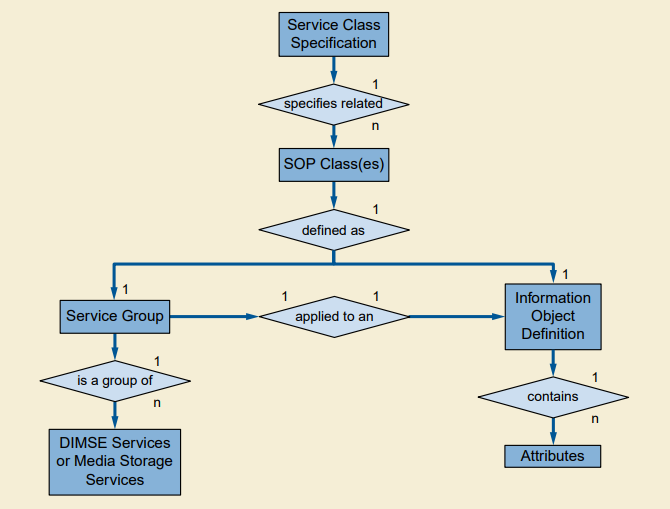
\includegraphics[width=\textwidth]{dicom-information-model}
\caption{Základní části informačního modelu DICONDE a vazby mezi nimi. \cite{dicom-standard}}
\label{fig:dicom-information-model}
\end{figure}

Jednou z částí informačního modelu je \zkratka{zk:IOD}, která slouží k objektově orientované abstrakci reálných objektů. IOD nereprezentuje konkrétní reálný objekt, ale pouze třídu reálných objektů, které sdílí stejné informace. Jinými slovy si lze IOD představit jako třídu, která je využívána v objektově orientovaných programovacích jazycích.

Další částí, kterou informační model DICOM definuje jsou služby. Služby umožňují DICOM aplikací provádět operace po síti, slouží tedy ke komunikaci. Hlavním využitím služeb je přenos a ukládání snímků v DICOM formátu. Vytvořením páru IOD-služba vzniká \zkratka{zk:SOP} třída. Aplikace definováním SOP tříd poskytuje ostatním DICOM aplikacím rozhraní, pomocí kterého definuje vlastnosti a možnosti aplikace. \cite{dicom-standard} 

Datový formát DICOM umožňuje zabalení dat, které jsou reprezentovány pomocí SOP instance do jednoho souboru. Kromě SOP instance se v souboru vyskytuje hlavička, která nese identifikační informace o zabalené SOP instanci. Hlavička se skládá ze 128 bytové preambule, 4 bytového DICOM prefixu a metadat. Metadata jsou kódována pomocí atributů. Strukturu DICOM souborů popisuje obrázek \ref{fig:dicom-file-structure}

\begin{figure}[htb]
\centering
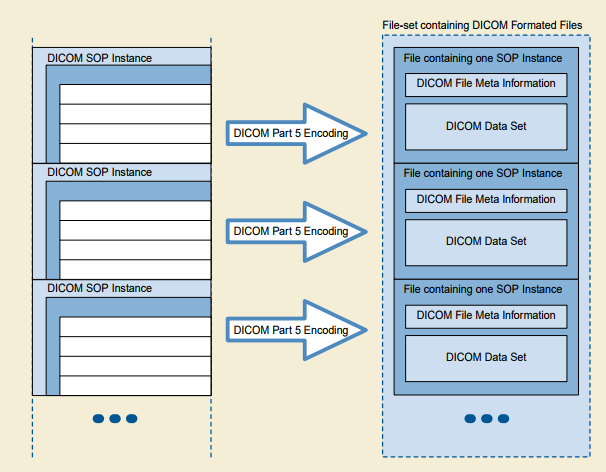
\includegraphics[width=\textwidth]{dicom-file-structure}
\caption{Struktura dat souboru v DICOM formátu. \cite{dicom-standard}}
\label{fig:dicom-file-structure}
\end{figure}

\paragraph{DICOM atributy} jsou základní entity pro tvorbu DICOM objektu. Každý DICOM atribut se skládá ze značky, datového typu, délky a hodnoty. Značka atributu definuje pomocí unikátního kódu typ atributu. Značka se skládá z dvou 2 bytových haxadecimálních čísel, kde první z čísel definuje skupinu atributu a druhé je unikátní číslo ve skupině. Datový typ je reprezentovaný pomocí dvou písmen, například unsigned short je zakódovaný jako US. Někdy swe stává, že informace o datovým typu je redundantní, protože datový typ je úzce spjat s typem atributu, nicméně je dobrou praxí datový typ vždy uvádět. Jako příklad atributu lze uvézt atribut typu počet pixelů na výšku s hodnotou 96, který je definovaný značkou $(0028, 0010)$, datovým typem US, hodnotou 96 a délkou 2.

\paragraph{DICOM objekt} si lze představit jako objekty využívané v objektově orientovaném programování nebo jako rozhraní umožňující výměnu dat mezi dvěma aplikacemi bez nutnosti znalosti druhé aplikace, ale pouze znalosti tohoto rozhraní. Každý DICOM objekt se skládá z několika modulů, které se skládají. DICOM objekt je definován pomocí datového modelu, který  
definuje informační entity, jako například pacient, studie, série nebo instance (snímek).

Datový model si lze představit jako relační databázový model. Třídy DICOM datového modelu jsou nazývány jako \zkratka{zk:SOP} a jsou definovány pomocí \zkratka{zk:IOD}. Každé IOD je definováno pomocí informačních entit, které jsou definovány pomocí modulů. Každý modul je definován pomocí atributů, jejichž podoba byla popsána výše. Jak moduly, tak atributy mohou být buď povinné nebo volitelné. Výsledný soubor definovaný pomocí IOD musí obsahovat všechny povinné moduly a jejich atributy a může obsahovat volitelné moduly a jejich atributy.

\paragraph{DICONDE} je standard pro ukládání a přenos snímků v nedestruktivní defektoskopii. Jedná se o rozšíření standardu DICOM pomocí harmonizační normy \cite{diconde-standard}. DICONDE předefinovává některé z DICOM modulů tím, že přejmenovává některé z atributů modulů nebo přidává nové privátní atributy. Díky tomu, že jsou měněny pouze názvy atributů a značky zůstávají stejné je zajištěna vzájemná kompatibilita formátů. Typickým příkladem změny názvu atributu může být například atribut se značkou $(0010,0010)$, který v případě DICOM náleží modulu Patient a v případě DICONDE modulu Component, který má v případě DICOM název Patient Name a v případě DICONDE Component Name. Stejným způsobem jsou pomocí harmonizační normy předefinovány DICOM moduly Patient, Patient summary a Patient study na DICONDE moduly Component, Component summary a Component study.

\paragraph{Implementace} standardu, případně datového formátu, DICOM je cílem několika projektů. Projekty lze rozdělit podle toho, zda implementují pouze datový formát nebo celý stadard včetně implementace služeb pro komunikaci s ostatními aplikacemi. Dostupné implementace popisuje tabulka \ref{dicom-comparsion}. Na základě této tabulky byla vybrána implementace Fellow Oak DICOM, která k implementaci využívá programovací jazyk C\# a splňuje .NET Standard 1.3 a vyšší. Implementovaná verze standardu DICOM je 2017c. Pro použití rozšířeného standardu DICONDE lze tuto knihovnu snadno rozšířit o atributy definované normou \cite{diconde-standard}.

\begin{table}[]
\centering
\caption{Srovnání formátu DICOM.}
\label{dicom-comparsion}
\rotatebox{90}{
\begin{tabular}{|l|l|l|l|l|}
\hline
Název            & Jazyk                           & DICONDE data format & DICOM standard & Licence \\ \hline
Fellow Oak DICOM & C\# / .NET Standard 1.3 a vyšší & ANO                 & ANO            & MS-PL   \\ \hline
dcm4che          & Ruby 1.9.3                      & ANO                 & ANO            & MPL 1.1 \\ \hline
MITK             & C++                             & ANO                 & ANO            & BSD     \\ \hline
pydicom          & Python 2.6 a vyšší              & ANO                 & NE             & -       \\ \hline
\end{tabular}}
\end{table}